\chapter{Design And Implementation} % - Design and Implementation
\label{chap:design}
%   - overview
%   - original tinkering and considerations
%   - features and considerations
%       - readline
%       - golang
%       - logging
%           - remote phoning home
%       - extensibility (markdown, parser)
%       - embedded files
%           - Template expansion
%           - Running examples
%       - usability 
%   - architecture of cli-tool
%   - architecture of web-tool
%       - how sandboxing is achieved

%docker daemon exposed over https for the sake of websockets. something the sdk cannot handle.

In this chapter, we will dive into the details surrounding the engineering of
the \textit{CLI-Tutor} tool, its supporting web application and the online
documentation tool. We will first start by sharing the approaches of some of
our early prototypes. We will discuss all the considerations and features that
shaped the architecture of \textit{CLI-Tutor}. Additionally, the technical
stack that \textit{CLI-Tutor} is built on will be introduced. This includes all
technical aspects of this work ranging from the core command line application,
\textit{CLI-Tutor}, to the servers and tools required to build our web
applications and perform our user study. A detailed discussion of the technical
aspects around some of the most important features in the current version of
\textit{CLI-Tutor} will then follow.  


\section{First Attempts} In the early stages of this thesis work, while
attempting to model the problem and develop the requirements for a technical
solution several prototypes were created. The early prototypes were written
in \textit{Python} \cite{python}. It was clear from an early stage that
\textit{readline} would be a mandatory element of any approach we would take. Early
attempts broadly focused on two different approaches:

\begin{itemize} \item An \textit{Expect}\cite{libes1995exploring} like
    approach. \textit{Expect} is an add-on to the \textit{Tcl} scripting
    language and is a way of writing scripted interactions with sub-processes.
    An \textit{Expect} script can be used to launch a sub-process and
    communicate with it, for each action expected results can be specified.
    \textit{Expect} scripts are popular for feigning user input and for testing
    or combining separate services. It is designed entirely with command line
    applications in mind and thus seemed a worthwhile approach for
    \textit{CLI-Tutor}, especially because we wanted to design lessons which
    had expected values and interactive exercises. Two prototypes were built
    using  \textit{Python} and \textit{Go}. The plan was to use \textit{Expect}
    to interact with a spawned \textit{Bash} sub-process. While initially
    promising, the \textit{Expect} approach was abandoned due to limitations in
    the libraries and concerns around being able to build an appropriate user
    interface to wrap \textit{Expect}.

    \item Creating and managing PTYs\footnote{PTY refers to a Linux
        pseudoterminal, the low-level interface through which terminal data
    flow is implemented in Linux.}. Prototypes integrating \textit{readline}
    implementations were built using this approach with some success. However,
    this approach necessitated intricate low-level programming and raw
    communication with the terminal. It was eventually deemed too complicated
    and operating system specific to be appropriate for \textit{CLI-Tutor}. 

\end{itemize}

    Other attempts included writing a GUI application to create a fake terminal
    environment. However, it was decided that a compiled command line
    application would be most appropriate for this purpose as it would allow us
    to capitalise on the existing interface of the user's terminal and the
    wealth of libraries and tools available to facilitate command line
    application development. Creating a mock shell environment and using
    operating system native system calls would be the most proper approach for
    \textit{CLI-Tutor}.

\section{Tools and Libraries}
\label{sec:tools}

\subsection{\textit{CLI-Tutor}}
\begin{itemize}
    \item \textit{readline} is the \textit{Go} port of the gnu readline
        \cite{ramey_fox_readline} line editing software. It forms the backbone
        of the lesson menu in \textit{CLI-Tutor}.

    \item \textit{bubbletea} is \textit{Go} framework for building stateful terminal
        applications using the \textit{Elm} Architecture\footnote{More on the \textit{Elm}
        Architecture here: \url{https://guide.elm-lang.org/architecture/}}.
        \textit{bubbletea} is a part of the charm\footnote{More on the charm
        project here: \url{https://charm.sh}} project, which is a host of
        frameworks and libraries aimed at modernising the command line
        interface. The project also includes a host of smaller libraries and
        extensions designed to be used with \textit{bubbletea}
        applications. \textit{bubbletea} is the TUI framework used to manage
        switching between the menu and lesson views in \textit{CLI-Tutor}.

        \begin{itemize}
            \item \textit{bubbles} is a collection of UI components to be used alongside \textit{bubbletea}.
            \item \textit{bubblezone} is a community-contributed extension to
                \textit{bubbles} components that allows for zones and hitboxes
                to be established in the user interface.
            \item \textit{lipgloss} is a styling and layout toolkit for \textit{bubbletea} applications.
        \end{itemize}

    \item \textit{glamour} is a terminal \textit{Markdown} rendering library also 
        created by the \textit{charm} team. It is used to display lesson tasks
        during a lesson in \textit{CLI-Tutor}.

    \item \textit{cobra} is a very popular CLI framework that is used in
        \textit{CLI-Tutor} for feature flags, the help menu and for managing
        start-up and clean-up behaviours.
        
    \item \textit{goldmark} is a \textit{Markdown} parser written in \textit{Go}. It is used in 
        \textit{CLI-Tutor} for parsing lesson files into data structures that
        drive the lesson interface and also for populating the menu with a list
        of available lessons.

    \item \textit{termenv}  is a \textit{Go} library used for managing terminal colours
        and environments. It is used in \textit{CLI-Tutor} for maximising
        compatibility across terminals, producing colours and for certain
        terminal controls such as screen clearing.
\end{itemize}

\subsection{Web Application}

\begin{itemize}
    \item \textit{Svelte} is a JavaScript/TypeScript frontend framework. It was
        chosen to be the frontend for our web application due to its
        simplicity, low learning curve and bundled output approach.

    \item \textit{Vite} is the JavaScript bundler used alongside Svelte to package the project for the web.

    \item \textit{XtermJs} is a terminal component for frontend applications.
        It is the default terminal in the exceptionally popular text
        editor VSCode\footnote{More about VSCode here:
        \url{https://code.visualstudio.com/}}. The terminal component is used
        alongside it's \textit{attach} add-on to form a connection over
        WebSockets to a \textit{docker} container. This is how sandboxed environments
        are provided over the web to users.

    \item \textit{Fiber} is the HTTP framework used to create the backend for
        our web application. It is primarily used as a proxy between the
        frontend and the \textit{docker daemon} running on our backend server.

    \item \textit{Docker SDK} is a first party \textit{Go} Software Development Kit
        (SDK) for interacting with the \textit{docker daemon}. It was chosen for
        interoperability with the backend HTTP framework which also uses \textit{Go}.

    \item \textit{MkDocs} is an industry-standard static site generator for
        documentation websites. It was used to create a documentation website
        for the user study conducted in this work.
        \begin{itemize}
            \item \textit{MkDocs-Material} is an extension to \textit{MkDocs}
                providing an attractive modern theme and some additional visual
                elements to the static documentation website created for
                \textit{CLI-Tutor}.
        \end{itemize}
\end{itemize}

\subsection{Server Infrastructure}
\begin{itemize}
    \item \textit{Linode} is a cloud service provider offering low-cost Virtual Private Servers. Two servers were used to implement the web application portion of \textit{CLI-Tutor}.
    \item \textit{Nginx} is a high performance web server. It was utilised on
        both our servers to serve as a reverse proxy to allow communication
        with \textit{docker} and our backend API.
    \item \textit{Gitlab CI/CD} is a Continuous Integration and Continue Delivery service used for testing, building and deploying our web application.
    \item \textit{Grafana Cloud} is a monitoring service. It was used in
        \textit{CLI-Tutor} to monitor uptime and for log agglomeration from our
        servers to ensure everything was running well.
\end{itemize}

\section{Features and Considerations of \textit{CLI-Tutor}}

\subsection{Why \textit{Go}?} The \textit{Go} programming language was selected
for \textit{CLI-Tutor} for numerous reasons. \textit{Go} is a popular language
for writing command line applications, with numerous modern CLI applications
such as the \textit{GitHub} CLI \cite{github_cli} and \textit{docker} CLI
\cite{dockerinc_2022}. This popularity in CLI applications also has the side
effect of there being a wide selection of libraries available for implementing
CLI interfaces (see: \autoref{sec:tools}). In addition to good tooling,
\textit{Go} programs are compiled and thus easier to distribute across
operating systems than interpreted alternatives such as \textit{Python}
programs. \textit{Go} also comes with a well-featured standard library with
diverse options for interacting with the operating system, a core requirement
of \textit{CLI-Tutor}.


\subsection{Shell Environment}

Development of \textit{CLI-Tutor} started with the implementation of a
shell-like environment. A  \textit{Go} specific
\textit{readline}\footnote{\url{https://pkg.go.dev/github.com/chzyer/readline}}
package was used to create a simple \textit{REPL}\footnote{Read Evaluate Print
Loop} as a proof of concept. The \textit{readline} library supported a custom
prompt and through the use of some system calls a functional prompt with a
working \textit{readline} environment was created. The next challenge was how
to structure, create and interact with lessons.

\subsection{Lessons}

The first task was to model a lesson in the form of a data structure that could
be used in the working shell environment we had created at this point. It was
decided that a lesson could be modelled as a container that contains a series of
tasks, which would be modelled as a separate data structure (see: \autoref{lst:types}).

\subsubsection{Anatomy of a Lesson}

A lesson has a title and description which are used to populate the menu screen
of \textit{CLI-Tutor}. Every task contains a title and description as well. The
title of a task is displayed in the task tracker and the description is the
actual textual content of a task. This content is either explaining a concept
to the user, displaying a diagram or prompting the user to input some commands.
The amount of tasks dictate the length of the lesson. The user can keep track
of their progress inside a lesson by the task tracker, which displays the title
of the lesson, and the current task as well as a progression counter. A user is free to
proceed back and forth through the lesson using the in-built commands
\textit{n/next} or \textit{p/prev} unless the task is marked as interactive. In
this case, the user must perform an interactive task such as running a specific
command relevant to the task at hand. This mechanism as well as the progress
tracker are showcased in \autoref{fig:tracker}.

% \vspace{1em}
\begin{listing}
    \begin{minted}{go}
type Lesson struct {
    Name        string
    Vocabulary  []string
    Description string
    Tasks       []Task
}

type Task struct {
    Title       string
    Description string
    Expected    string
}
    \end{minted}
    \caption{Data structures for a Lesson and a Task within a Lesson.}
    \label{lst:types}
\end{listing}

\begin{figure}[htbp]
	\centering
	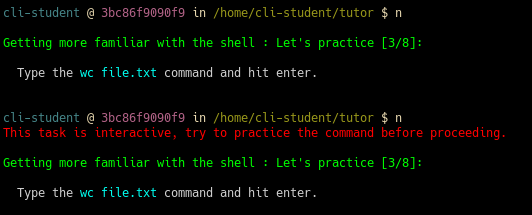
\includegraphics[width=0.8\textwidth]{img/tracker}
	\caption{Screenshot of the progress tracker and interactive task feature.}
	\label{fig:tracker}
\end{figure}
\clearpage

\subsubsection{Specifying Lessons}
% \vspace{-3em} %TODO: Figure out this float issue.

The first versions of a \textit{CLI-Tutor} lesson were written directly in
\textit{Go} source code. Not only was this tedious but also extremely specific
to this implementation; rendering extensibility and open-source contributions
difficult. It was decided that some sort of data exchange or markup language
would be more appropriate for specifying lessons. Early considerations included
\textit{JSON}\footnote{JavaScript Object Notation. See:
\url{https://www.json.org/json-en.html}} and \textit{YAML}\footnote{Yet Another
Markup Language. See \url{https://yaml.org/}}. These solutions proved to be
difficult to work with in terms of formatting and did not make the process of
contributing lessons any easier for an external contributor.

Ultimately, the decision to implement the lessons in \textit{CommonMark
Markdown}\footnote{A popular implementation of \textit{Markdown}. See:
\url{https://commonmark.org/}} was taken. \textit{Markdown} was a pragmatic
decision due to its ubiquity in the software development space and abundance of
parsers. Furthermore, \textit{Markdown} allowed us to specify our formatting
directly in the lesson document and made for a source code free template for
specifying lessons.

\subsection{Lesson Parsing}
\label{sec:parser}

Once \textit{Markdown} was decided to be the implementation language for our
lessons the next step was to populate our lesson-related data structures (see:
\autoref{lst:types}) in order to drive the tutorial program. To achieve this a
structure for specifying a lesson had to be created. After the specification
was complete, a parser had to be written. The \textit{goldmark} markdown parsing
library for \textit{Go} was selected. This library allowed us to create a
custom parser for our lesson files. The parser first parses a selected lesson
file into an \textit{AST} (Abstract Syntax Tree). Once this tree is created, it
is traversed using a \textit{Depth First Search} as a means to navigate to all
the different syntax nodes in the tree. In our lesson file specification, we
make divisions using heading weights in our \textit{Markdown} files. 

Level 1 headings and their subsequent nested text are used for
\textit{Lesson}\footnote{\textit{Lesson} and \textit{Task} in this
capitalised and italicised form refer to our \textit{Lesson} and \textit{Task}
data structures (see: \autoref{lst:types}).} level data, specifically the
lesson's title and description. 

Each subsequent level 2 heading refers to an individual \textit{Task}. The text
nested in between the level 2 headings belongs to the \textit{Task} above the text.
\textit{Markdown} elements such as code blocks and inline code snippets are
used to stylise text during the lesson. The expected value feature of
\textit{Task}s is implemented using the quotation element (\textit{>})
of \textit{Markdown}. As the traversal of the \textit{AST} continues
\textit{Task}s are appended to the \textit{Tasks} array in the \textit{Lesson}
data structure. This creates the series of tasks in the lesson, which are
eventually navigated through by iterating this \textit{Tasks} array. 

Level 3 headings are used to define the lesson's vocabulary or set of permitted
commands. There are additional features such as the nature of how interactive
task values are to be calculated that can also be specified in the lesson file.
For a full \textit{Markdown} specification of a \textit{CLI-Tutor} lesson, see:
\autoref{lst:markdown} and for the implementation of the custom parser see:
\autoref{lst:parser}. 

\subsubsection{Template Expansion}

There is actually one step that takes place just before the parsing of a
lesson. This is where values can be interpolated into the \textit{Markdown}
files using \textit{Go}'s powerful in-built template\footnote{\textit{Go}
    standard library documentation: \url{https://pkg.go.dev/text/template}}
    library. This allows for special system-specific or environment-specific
    values to be interpolated into a lesson at the time of parsing, allowing
    for even more personalised explanations to be baked into the lessons. An
    example of this is demonstrated in \autoref{fig:templateexpansion} where
    user and system-specific information is presented in the explanation of a
    shell command prompt. This allows for lessons to be less static and further
    capitalises on the opportunities available in interactive programs compared
    to written documentation.

\begin{figure}[htbp]
	\centering
	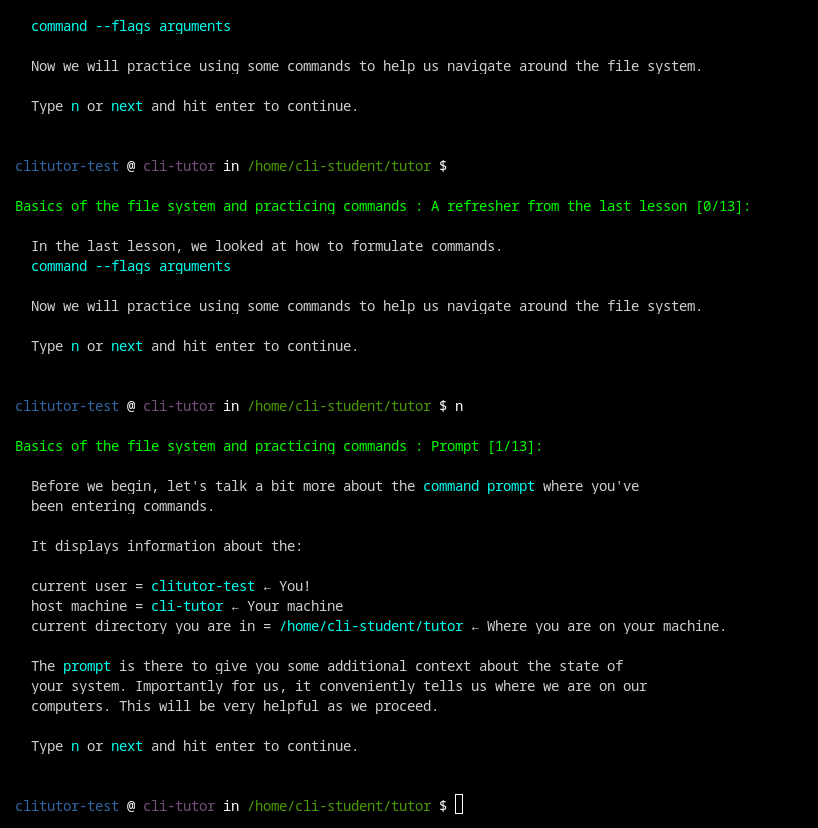
\includegraphics[width=1\textwidth]{img/cliexpansionfull}
	\caption{Screenshot of a \textit{CLI-Tutor} lesson showing values interpolated into the lesson.}
	\label{fig:templateexpansion}
\end{figure}

\subsubsection{Running Examples}

Another feature of \textit{CLI-Tutor} is the inclusion of certain files that
are created on the user's file system for the duration the tutor program is
running. These files serve as running examples and allow for lessons that use
real files and data to be crafted. This allows for more creativity and
opportunities for engaging the user's when creating interactive tasks.

\begin{figure}[htbp]
	\centering
	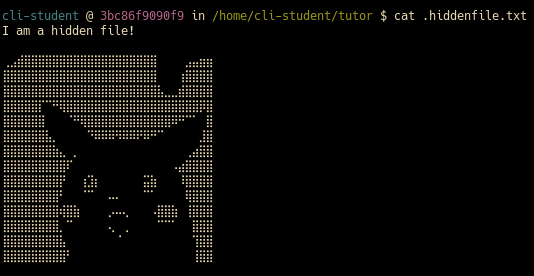
\includegraphics[width=0.8\textwidth]{img/hidden}
    \caption{Screenshot of a hidden file created by the \textit{CLI-Tutor} as an interactive example.}
	\label{fig:hidden}
\end{figure}

 
\subsection{Embedded Files}

The two previous features in addition to the goal of being able to distribute
\textit{CLI-Tutor} as a single executable binary necessitated the inclusion of
both lesson files and files that serve as running examples into the compiled
binary. This was achieved using a compiler directive recognised by the \textit{Go}
compiler named \textit{go:embed}\footnote{\url{https://pkg.go.dev/embed}}. This
allowed for the creation of a virtual file system for the program to be able to
read files as if it were a real file system. Embedding files directly into
the program also greatly contributes towards the ease of distribution and
contribution of \textit{CLI-Tutor} as all the parts that make up the tutor reside
in one codebase.

\subsection{User Interface}

The user interface of \textit{CLI-Tutor} is divided into two main views, the
lesson view and the menu view. The default view and what the user is presented with
upon launching \textit{CLI-Tutor} is the menu view. The menu is populated using
a variation of the parser described in \autoref{sec:parser}. As previously
mentioned, \textit{CLI-Tutor} is a TUI application. To manage the two distinct
views and provide interactive user interface elements the \textit{Bubbletea}
library was used. \textit{Bubbletea} is a library for making Textual User
Interfaces and is inspired by the \textit{Elm} architecture. The \textit{Elm}
architecture is a pattern that consists of three-part structure where messages
are sent between parts to alter state, update the user interface and act upon
messages.

\subsubsection{The \textit{Elm} Architecture applied to \textit{CLI-Tutor}} 

The \textit{Elm} architecture's three main parts are:

\begin{itemize}
    \item \textit{Model:} The model controls the state of the application. The 
        \textit{CLI-Tutor} tool uses three models to manage its state. The
        \textit{MainModel} is, as the name suggests, the main controller and
        houses the models for the menu view and the lesson view inside it. The
        job of the \textit{MainModel} is to present the correct view to the
        user and to process all the different messages that can be sent back
        from the lesson and menu models. The selection of views is done by the \textit{state} member of the \textit{MainModel}.  The definitions of the three models in \textit{CLI-Tutor} can be found in \autoref{lst:model}.

\begin{listing}
\begin{minted}{go}
const (
	menuView sessionState = iota
	lessonView
)

type MainModel struct {
	state      sessionState
	menu       tea.Model
	lesson     tea.Model
	quitting   bool
	windowsize tea.WindowSizeMsg
}

type MenuModel struct {
	list       list.Model
	choice     string
	quitting   bool
	windowsize tea.WindowSizeMsg
}

type LessonModel struct {
	currentLesson lesson.Lesson
	rl            *readline.Instance
	r             *glamour.TermRenderer
	quitting      bool
}
\end{minted}
    \caption{Models used to build the user interface of \textit{CLI-Tutor}.}
    \label{lst:model}
\end{listing}

\item \textit{Update:} This a method that is implemented for a model. The
    \textit{Update} method consumes the messages sent around between the
    components of a system built on the \textit{Elm} architecture. The update
    function can then manipulate the state of its corresponding model to create
    reactivity. Messages are events generated through interaction with the
    application and actions such as resizing a window. In \textit{CLI-Tutor},
    messages are used to communicate the size of the terminal, manage key
    presses, enable selections in the menu and handle quitting the application.
    A message-based architecture allows for a lot of flexibility in terms of
    defining custom messages that can trigger other behaviours or make state
    changes. An example is parsing a lesson after it is selected in the menu
    view and assigning it as the current lesson in the lesson view.

\item \textit{View:} The \textit{View} is the last part of the \textit{Elm}
    architecture and is responsible for rendering the visual environment based
    on the state of its related \textit{Model}. In \textit{CLI-Tutor}, the view
    is only used for the menu view of the application. It cannot be used in the
    lesson view due to the implementation of the \textit{readline} library,
    which consists of a blocking \textit{for} loop. To get around this we
    block the \textit{Elm} update loop for the duration of the lesson with the
    \textit{readline} loop. When a lesson is completed or the user elects to
    quit the lesson, the \textit{readline} loop breaks and an exit message is
    sent to the \textit{Update} method \textit{MainModel} signifying the change
    of state from lesson to menu. This update then triggers a state change on
    the \textit{MainModel} which results in the user being presented with the
    menu view. Because the state is kept throughout the run time of the
    application the menu will still have the lesson the user selected
    highlighted, enhancing the user experience.

\end{itemize}

\subsubsection{Markdown Renderer}

We mentioned how we parse the lesson Markdown files in \autoref{sec:parser}. As
lines of \textit{Markdown} are parsed they are stored as raw byte arrays in the
\textit{Lesson} and \textit{Task} data structures. This has the desired side
effect of maintaining the formatting inherently coded into a \textit{Markdown}
document. When it comes time to display this information during a lesson, a
terminal \textit{Markdown} renderer named \textit{glamour} is used. Rendered
text to the terminal is both styled and formatted by \textit{glamour} resulting
in a near direct translation between the lesson file and what is displayed to
the user in the terminal. Using a \textit{Markdown} renderer also gave us the
flexibility of specifying custom styling on all the different \textit{Markdown}
style elements and to fine-tune the look and feel of lessons by tweaking the
style sheet being used by the renderer.

\subsection{Validation}

In the interest of building interactivity into our lessons, we needed to have a way of
validating the inputs and actions of our users. Our input validation mechanism
is incorporated into the \textit{readline} loop of the lesson view in
\textit{CLI-Tutor}. Every time the user issues a command by hitting enter, the
string the user entered at the command prompt is sent through a validation
cycle. The first step is checking whether the string matches one of the many
in-built special commands. These commands do things like proceed back and forth
through the lesson, quit the lesson, print out a list of available commands and
toggle \textit{zen-mode}. If the string is not one of these special commands
then it is assumed that the user is attempting to issue a system or shell
command. For convenience, input strings at this point are stripped of white space and split into an array
to examine the individual tokens that make up the whole command. The next steps are:

\begin{itemize}

    \item Checking whether the specified command is in the current lesson's
        vocabulary and thus permitted to be run. This is done by checking the
        very first token of the string. Any tokens following the special shell
        operators \textit{|} and \textit{\&} are also validated. If the command
        passes this stage it means the string contains commands valid and
        permitted in the current lesson.


    \item After passing initial validation, further checks are performed to
        prevent the user from running into permissions issues or working in a
        sensitive root or system directory. The command also checks for
        certain special conditions that need to be accounted for. Special
        conditions such as:

        \begin{itemize}
            \item Several commands chained as pipes.
            \item The presence of logical operators such as \textit{||} and \textit{\&\&}.  
            \item Whether the command has arguments or flags specified.
            \item Whether the command launches an external command like a
                pager, which would require a redirection of the spawned
                sub-process's standard input and output streams to those of
                \textit{CLI-Tutor}.  
        \end{itemize}

        Each of these cases requires special handling in the way the system
        call is placed. The correct method is selected at this point and a
        system call is issued.

    \item At this stage the issued command is stored in a variable that tracks
        the last issued command. This is necessary to support the
        repeat previous command or \textit{!!} shell operation.

    \item The next step is to return the combined output of the issued
        commands standard out and error streams to the user interface. In the
        case that the command was an interactive sub-process like a pager, the
        streams of the sub-process and redirected to the user interface at this
        point.

    \item A final step is to check where the current \textit{Task} has a
        defined expected value. If this is the case the returned output of the
        issued command is compared to this expected value and the appropriate
        success or failure feedback is provided to the user. If the user
        successfully completed the task the tutor automatically increments the
        task tracker, resulting in the user being automatically advanced to the
        next task in the lesson.


\end{itemize}

\subsection{Logging}

To assist with gathering usage data and user behaviour, \textit{CLI-Tutor}
maintains a log file which can be optionally sent back to a server for
examination. The log file is a mirror copy of the lesson session with
timestamps for every action that occurs during the lesson.

This feature is on by default during the user study phase of this work but can
be opted out of with a flag that can be supplied when launching
\textit{CLI-Tutor}. The purpose of this feature is entirely in support of the
user study conducted in this thesis work and the feature will likely be removed
from the tool upon the conclusion of this work.

\section{Web Application}

As previously mentioned, the core of \textit{CLI-Tutor} is the command line
application described in the previous section. The accompanying web application
was created with the goal of simplifying the distribution of the tool and
organising the user study. While not originally a design requirement, the idea
of sandboxing our application proved very attractive, especially given the
nature of our subject matter. While this kind of sandboxing would be easy to
achieve with tools such as \textit{docker} or virtual machines. It is too much
to expect a novice user to set up and diminishes the potential user base of
\textit{CLI-Tutor}. Creating a web application also relaxes the cross-platform
compatibility concerns of building an application that interacts directly with
the operating system, like a shell.


\subsection{Frontend} The frontend is a simple JavaScript web application
written in Svelte. Svelte proved to be a good choice due to its simplicity,
small bundle size and developer ergonomics. TypeScript was the main language of
development when it came to the frontend. The main role of the frontend
application is to provide some instructions and to present the user with a
special frontend terminal component. This terminal component is from the
popular library \textit{Xterm.js}. This terminal emulation solution was chosen
due to its proven robustness as the default terminal in the \textit{VSCode}
text editor and due to a first-party add-on that makes it possible to attach
the terminal component over the WebSocket\footnote{A full-duplex communication
protocol native to modern web browsers.} protocol to the interactive
\textit{docker} container(see: \autoref{fig:webversion}). The process of
provisioning, connecting and cleaning up to \textit{docker} containers is
facilitated through the use of API\footnote{Application Programming Interface}
calls to a backend running on the same server. 

\subsection{Backend} The backend is a REST\footnote{Representational state
transfer: An architectural style for creating interfaces to allow Client-Server
communication.} API, written in \textit{Go} using the \textit{Fiber} library.
The API allows the frontend to communicate with the \textit{docker daemon} also
running on the same server. Container creation, deletion and resizing of the
containers \textit{PTY}\footnote{This is necessary to sync the size of the pty
created in the frontend terminal with the interactive \textit{docker}
container's terminal running on the server.} are handled by this backend API
using the \textit{docker} SDK for \textit{Go}; which interacts directly with
the \textit{docker daemon} running on the server. The attaching over
\textit{WebSockets} of the frontend to the spawned docker container is achieved
through an API call directly to the \textit{docker daemon} using the
container's id which is received in a response message from the container
creation API endpoint.

\subsection{\textit{Docker Daemon}} To facilitate the sandboxing via
\textit{docker}, the \textit{docker daemon} is exposed over
\textit{TCP}\footnote{Transmission Control Protocol} with
\textit{TLS}\footnote{Transport Layer Security}. This allows for a direct
connection over \textit{WebSockets} to be negotiated between the frontend user
interface and the \textit{docker} container running \textit{CLI-Tutor}. For
safety and consistency with how the backend API is accessed, the \textit{docker
daemon} is accessed via reverse proxy using the \textit{Nginx} web server which
manages all incoming \textit{HTTP(S)}\footnote{Hypertext Transfer Protocol
(Secure)} connections to the server. 

 
\subsection{CLI Only} As mentioned earlier, a CLI-only version (see:
\autoref{fig:cliversion}) was also created using essentially the same
architecture as the version that includes \textit{CLI-Tutor}. Slight visual
differences were made to differentiate the two however they are based on
fundamentally the same \textit{docker} image, with the only difference being
that the "CLI Only" version does not contain the \textit{CLI-Tutor} tool and
drops the user directly into a Linux shell. The CLI-only version also contains
an additional button for navigating to the documentation website.

\subsection{Documentation Website} Created using MkDocs,\cite{mkdocs} a widely
used tool for documentation in the software development world. The
documentation website (see: \autoref{fig:docsweb}) was built to support the
User Study. It uses the same lessons as in the \textit{CLI-Tutor} application,
albeit with some prompts for user interface actions removed. The fact that the
lessons in \textit{CLI-Tutor} are implemented in \textit{Markdown} made
creating web pages out of the files straightforward.

\subsection{Monitoring}

A monitoring stack using \textit{Grafana} was also set up on the web servers.
This was done to monitor performance, availability and to facilitate
the debugging of any potential issues. Log agglomeration was also performed
with \textit{Loki}\footnote{Log agglomeration tool in the \textit{Grafana}
monitoring stack} and \textit{Promtail}\footnote{The server side agent used by 
    \textit{Loki} to scrape system logs.}, the latter of which was run in a
    separate docker container. This information was forwarded to the
    \textit{Grafana Cloud} web interface.

\section{Extending CLI-Tutor}
%TODO: Check if the "following page" thing holds true in the final version of
%the paper

The extensibility of \textit{CLI-Tutor} has been a priority since the inception
of the tool. This is a key factor for the longevity and usefulness of the tool
beyond this thesis work. \textit{CLI-Tutor} is open source and hosted in public
repositories under a \textit{MIT}\cite{mitlicense} license. Contributing
lessons to \textit{CLI-Tutor} is uncomplicated owing to the use of
\textit{Markdown} files to specify lessons. On the following page, we provide a
complete specification and readable example of all the features available
during lesson creation and supported by \textit{CLI-Tutor}'s lesson parse, at
the time of writing (see: \autoref{lst:markdown}).


\begin{listing}
\begin{minted}{markdown}
# Lesson Title

A line under a level 1 heading is the lesson description. This is also
displayed in the menu.

## First Task Title

Task instructions are parsed as normal lines under a level 2 heading.

Even line breaks and nested elements will reflect in the lesson. This
greatly enhances readability.

`Commands` are highlighted with backticks.

Text can be injected into a lesson at the time of parsing with template
functions like this --> {{SomeFunc}}

## Second Task Title

This is the first line following a second level 2 heading and thus the text
of task #2.

```
Code blocks can also be used to represent larger blocks of instructions or
for ASCII diagrams.
```
## Interactive tasks with expected values

If the current task is expecting a certain output to a command the user 
types, we can specify that using the `>` syntax.

> {{TestFunc}}

## Runtime expected value calculation

Sometimes the correct value for a given task can only be computed at run 
time, to achieve this we can specify the expected value of a task to 
be the output of a system call by prepending a `!` and then the expected
command.

> !ls -la

### Lesson Vocabulary (Provided as a comma-separated list of values under a level 3 heading )

vim, ls, cp, cat, echo <--- only these commands will be permitted in this lesson.
\end{minted}
    \caption{Specification for Markdown lesson files.}
    \label{lst:markdown}
\end{listing}
